\documentclass[journal]{vgtc}                     % final (journal style)
%\documentclass[journal,hideappendix]{vgtc}        % final (journal style) without appendices
%\documentclass[review,journal]{vgtc}              % review (journal style)
%\documentclass[review,journal,hideappendix]{vgtc} % review (journal style)
%\documentclass[widereview]{vgtc}                  % wide-spaced review
%\documentclass[preprint,journal]{vgtc}            % preprint (journal style)


%% Uncomment one of the lines above depending on where your paper is
%% in the conference process. ``review'' and ``widereview'' are for review
%% submission, ``preprint'' is for pre-publication in an open access repository,
%% and the final version doesn't use a specific qualifier.

%% If you are submitting a paper to a conference for review with a double
%% blind reviewing process, please use one of the ``review'' options and replace the value ``0'' below with your
%% OnlineID. Otherwise, you may safely leave it at ``0''.
\onlineid{0}

%% In preprint mode you may define your own headline. If not, the default IEEE copyright message will appear in preprint mode.
%\preprinttext{To appear in IEEE Transactions on Visualization and Computer Graphics.}

%% In preprint mode, this adds a link to the version of the paper on IEEEXplore
%% Uncomment this line when you produce a preprint version of the article 
%% after the article receives a DOI for the paper from IEEE
%\ieeedoi{xx.xxxx/TVCG.201x.xxxxxxx}

%% declare the category of your paper, only shown in review mode
\vgtccategory{Research}

%% please declare the paper type of your paper to help reviewers, only shown in review mode
%% choices:
%% * algorithm/technique
%% * application/design study
%% * evaluation
%% * system
%% * theory/model
\vgtcpapertype{please specify}

%% Paper title.
\title{ggdist: Visualizations of Distributions and\\Uncertainty in the Grammar of Graphics}

%% Author ORCID IDs should be specified using \authororcid like below inside
%% of the \author command. ORCID IDs can be registered at https://orcid.org/.
%% Include only the 16-digit dashed ID.
\author{%
  \authororcid{Matthew Kay}{0000-0001-9446-0419}
}

\authorfooter{
  %% insert punctuation at end of each item
  \item
  	Matthew Kay is with Northwestern University.
  	E-mail: mjskay@northwestern.edu
}

%% Abstract section.
\abstract{%
  The grammar of graphics is ubiquitous, providing the foundation for a variety of popular visualization tools and toolkits. Yet support for uncertainty visualization in the grammar graphics—beyond simple variations of error bars, uncertainty bands, and density plots—remains scarce. Research in uncertainty visualization has developed a rich variety of improved uncertainty visualizations, most of which are difficult to create in existing grammar of graphics implementations. \textit{ggdist}, an extension to the popular \textit{ggplot2} grammar of graphics toolkit, is an attempt to rectify this situation. \textit{ggdist} unifies a variety of uncertainty visualization types through the lens of distributional visualization, allowing functions of distributions to be mapped to directly to visual channels (aesthetics), making it straightforward to express a variety of (sometimes weird!) uncertainty visualization types. This distributional lens also offers a way to unify Bayesian and frequentist uncertainty visualization by formalizing the latter with the help of confidence distributions. In this paper, I offer a description of this uncertainty visualization paradigm, and a retrospective and lessons learned from its development and adoption: \textit{ggdist} has existed in some form for about six years (originally as part of the \textit{tidybayes} R package for post-processing Bayesian models), and it has changed substantially over that time, with several rewrites and API re-organizations as it changed based on user feedback and expanded to cover increasing varieties of uncertainty visualization types. Ultimately, given the huge expressive power of the grammar of graphics and the popularity of tools built on it, I hope a catalog of my experience with \textit{ggdist} will provide a catalyst for further improvements to formalizations and implementations of uncertainty visualization in grammar of graphics ecosystems. % filler text. Replace with your abstract.
  %
  %% We recommend that you link to your supplemental material here in the abstract, as well
  %% as in the Supplemental Materials section at the end.
  
  A free copy of this paper and all supplemental materials is available at \href{https://github.com/mjskay/ggdist-paper}{https://github.com/mjskay/ggdist-paper} and is archived on Zenodo at \href{https://doi.org/10.5281/zenodo.7770984}{doi:10.5281/zenodo.7770984}.
}

%% Keywords that describe your work. Will show as 'Index Terms' in journal
%% please capitalize first letter and insert punctuation after last keyword
\keywords{Uncertainty visualization, probability distributions, confidence distributions, grammar of graphics}

%% A teaser figure can be included as follows
\teaser{
  \centering
  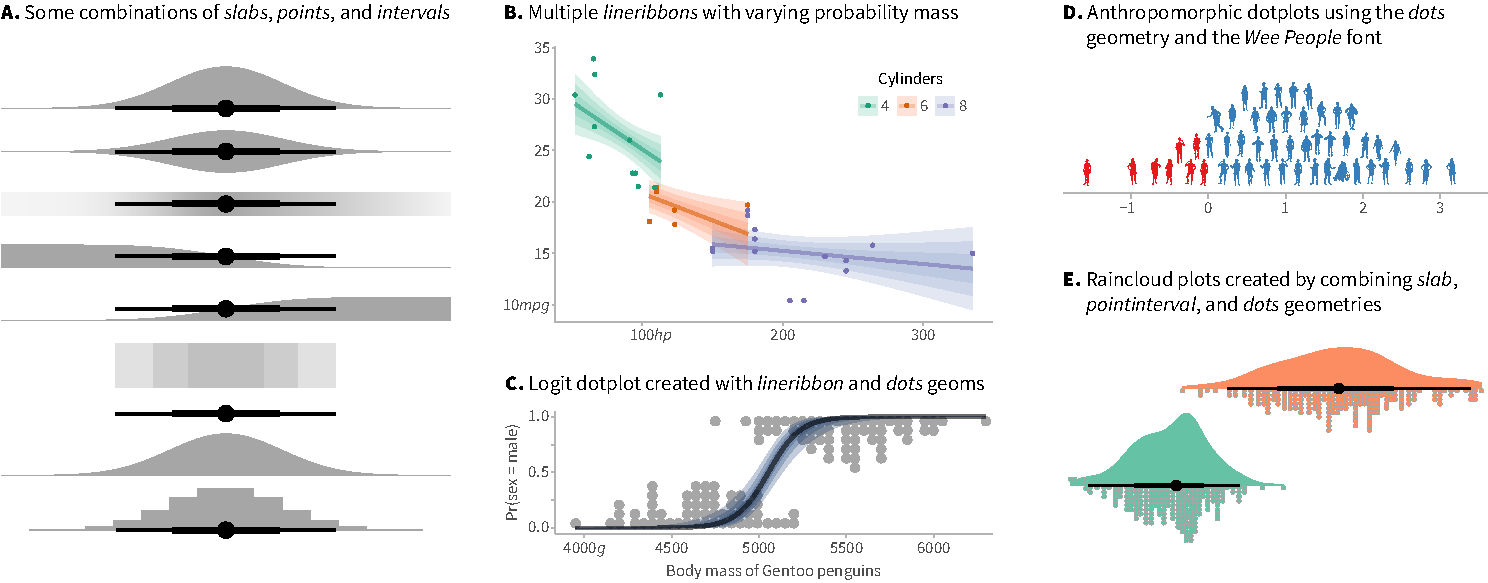
\includegraphics[width=\linewidth]{figs/teaser.pdf}
  \caption{%
  	Examples from the three major classes of geometries in \textit{ggdist}: \textbf{(A)} \href{https://mjskay.github.io/ggdist/articles/slabinterval.html}{slabintervals}, such as density plots, \textsc{cdf}s, intervals, and gradient plots; \textbf{(B)} \href{https://mjskay.github.io/ggdist/articles/lineribbon.html}{lineribbons}, such as uncertainty bands and fan charts; and \textbf{(D)} \href{https://mjskay.github.io/ggdist/articles/dotsinterval.html}{dots}, such as dotplots and beeswarm charts. Myriad combinations of these are possible, leading to charts like \textbf{(D)} \href{https://lnalborczyk.github.io/post/glm/}{\textit{logit dotplots}} and \textbf{(E)} \textit{raincloud plots}~\cite{allen2019raincloud}.%
  }
  \label{fig:teaser}
}

%% Uncomment below to disable the manuscript note
%\renewcommand{\manuscriptnotetxt}{}

%% Copyright space is enabled by default as required by guidelines.
%% It is disabled by the 'review' option or via the following command:
%\nocopyrightspace


%%%%%%%%%%%%%%%%%%%%%%%%%%%%%%%%%%%%%%%%%%%%%%%%%%%%%%%%%%%%%%%%
%%%%%%%%%%%%%%%%%%%%%% LOAD PACKAGES %%%%%%%%%%%%%%%%%%%%%%%%%%%
%%%%%%%%%%%%%%%%%%%%%%%%%%%%%%%%%%%%%%%%%%%%%%%%%%%%%%%%%%%%%%%%

%% Tell graphicx where to find files for figures when calling \includegraphics.
%% Note that due to the \DeclareGraphicsExtensions{} call it is no longer necessary
%% to provide the the path and extension of a graphics file:
%% \includegraphics{diamondrule} is completely sufficient.
\graphicspath{{figs/}{figures/}{pictures/}{images/}{./}} % where to search for the images

%% Only used in the template examples. You can remove these lines.
\usepackage{tabu}                      % only used for the table example
\usepackage{booktabs}                  % only used for the table example
\usepackage{lipsum}                    % used to generate placeholder text
\usepackage{mwe}         % used to generate placeholder figures
\usepackage{amsmath}
\usepackage{amssymb}
\usepackage{verbatim}
\usepackage{varwidth}

%% We encourage the use of mathptmx for consistent usage of times font
%% throughout the proceedings. However, if you encounter conflicts
%% with other math-related packages, you may want to disable it.
\usepackage{mathptmx}                  % use matching math font

\newenvironment{centerverbatim}{%
  \hfill\break
  \small
  \centering
  \varwidth{\linewidth}%
  \verbatim
}{%
  \endverbatim
  \endvarwidth
  \par
  \hfill\break
}

\begin{document}

%%%%%%%%%%%%%%%%%%%%%%%%%%%%%%%%%%%%%%%%%%%%%%%%%%%%%%%%%%%%%%%%
%%%%%%%%%%%%%%%%%%%%%% START OF THE PAPER %%%%%%%%%%%%%%%%%%%%%%
%%%%%%%%%%%%%%%%%%%%%%%%%%%%%%%%%%%%%%%%%%%%%%%%%%%%%%%%%%%%%%%%

%% The ``\maketitle'' command must be the first command after the
%% ``\begin{document}'' command. It prepares and prints the title block.
%% the only exception to this rule is the \firstsection command
\firstsection{Introduction}

\maketitle


%% \section{Introduction} %for journal use above \firstsection{..} instead

The grammar of graphics~\cite{wilkinson2012grammar} is ubiquitous, providing the foundation for a variety of visualization toolkits. Yet support for uncertainty visualization in grammar graphics implementations, generally speaking, remains rudimentary. Popular implementations like \textit{ggplot2}~\cite{wickham2010layered,wickham2011ggplot2} and \textit{Vega-lite}~\cite{satyanarayan2016vega} typically provide versions of error bars (for points), uncertainty bands (for lines), boxplots, and density plots. However, research in uncertainty visualization has developed a rich variety of alternative uncertainty representations, often designed to address shortcomings in those existing visualization types. Examples include, but are not limited to, quantile dotplots~\cite{kay2016ish,fernandes2018uncertainty}, gradient error bars~\cite{correll2014error}, gradient plots~\cite{bowman2019graphics,jackson2008displaying}, fan charts~\cite{jackson2008displaying}, and innumerable variations on eye plots~\cite{helske2021can,kay2016ish,barrowman2003raindrop,spiegelhalter1999surgical}. Yet, most of these alternative representations are---simply put---painful to convince existing grammar of graphics implementations to produce.

\textit{ggdist} is an attempt to rectify this situation. It started under the guise of \textit{tidybayes}---an R package I wrote for post-processing Bayesian models for use with \textit{ggplot2}---in about 2016. \textit{tidybayes} slowly gained some use in the Bayesian statistics community, but the package always had two complementary, but not perfectly aligned, use cases: post-processing Bayesian model output for visualization, and creating uncertainty visualizations in the grammar of graphics. The latter is bigger than \textit{just} Bayesian statistics: everyone needs to visualize uncertainty!\footnote{And, contrary to popular opinion---as we'll see later---Bayesian and frequentist uncertainty visualization can in fact be done within the same framework.} Recognizing this broader need, in 2020 I spun off the uncertainty visualization components of \textit{tidybayes} into a new package, \textit{ggdist}, and published it to CRAN. Since then it has steadily grown in use inside and outside the Bayesian statistics community in R, and now averages about 14,000 downloads per month (best described as ``modest'' for an R package).

\textit{ggdist} aims to be (1) a coherent extension to the grammar of graphics that makes it easy to create a variety of uncertainty visualizations, and (2) an implementation of a particular formalism for describing uncertainty visualizations: mappings of functions of distributions (e.g. densities) onto aesthetics (e.g. color). My ambition is that not only should that formalism be able to express a variety of uncertainty visualizations through a single coherent framework, but that that framework should be complete enough that someone else can wander along and express new uncertainty visualization types I've never thought of before (emphasis on \textit{I}---I think a formalism and its corresponding \textsc{api} truly shows its power when people make things with it that its creator has never thought of before). Naturally this is hard to demonstrate, but I will attempt to do so by giving a tour of \textit{ggdist} through recreations of a variety of uncertainty visualizations in the literature. Along the way, I'll also discuss lessons I've learned in how to effectively integrate uncertainty visualization into the grammar of graphics.

%I'll do this by grounding the design of \textit{ggdist} in a formal representation of uncertainty through mappings of functions of distributions onto visual channels or \textit{aesthetics}, and then show how this framework is able to recreate a wide variety of uncertainty visualization types from the literature.
%Over the course of its continuing development, I have learned a lot about how to integrate uncertainty visualization into the grammar of graphics. 

Ultimately, in the spirit of recent retrospectives on visualization system design~\cite{satyanarayan2019critical}, I hope to distill down some of what I've learned developing a moderately-well-used uncertainty visualization toolkit.\footnote{In the spirit of this being a retrospective, I'm keeping the tone informal. I think that's more honest; besides, after two years of a pandemic, I at least need a break from stilted academic writing. I hope you do too! If not, my condolences.} 
%. As time is a straight arrow, I can't provide direct evidence that there are visualization types I've never seen before that can be created with \textit{ggdist}, but I will describe instances in which I have encountered uncertainty visualizations in the literature and subsequently realized they were straightforward to express in \textit{ggdist}.
Given the huge expressive power of the grammar of graphics and the popularity of tools built on it, I hope a catalog of my experience might provide a catalyst for improved implementations of uncertainty visualization to flourish in existing grammar of graphics ecosystems, and ultimately for even better formal descriptions of uncertainty visualization to arise. Let's give it a try.

\section{Setting the stage}

\subsection{A simplified notation for the grammar of graphics}

To be able to talk more generally than a specific grammar of graphics implementation, we'll at least need a formal way of writing down visualization specifications separated from a particular implementation. I'll adopt here a notation that I've found works pretty well when I teach the grammar of graphics to undergraduates. I've used a variation on this notation when teaching \textit{ggplot2}, \textit{Vega-lite}, \textit{Altair}, and \textit{Tableau} and found students pick it up easily, which is at least some evidence it might be easy for folks to understand. The core notation describes a visualization in terms of its \textit{data variables}, \textit{aesthetic mappings}, and \textit{geometries}. We create a scatterplot, for example, by mapping one variable onto the \textit{x} aesthetic and another onto the \textit{y} aesthetic:\footnote{I am aware it is traditional to slap a number on each figure and float it off into a random corner of the page. I violate that norm throughout this paper without remorse.}

\hfill\break
\noindent
  \begin{minipage}{.5\columnwidth}
    \begin{align*}
\mathit{weight} &\rightarrow x\\
\mathit{mpg} &\rightarrow y\\
\textsc{geom} &= \mathit{point}
\end{align*}
  \end{minipage}%
  \begin{minipage}{.4\columnwidth}
    \centering
    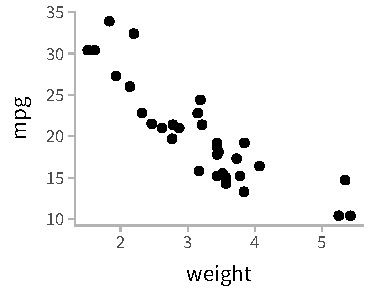
\includegraphics[width=1.2\columnwidth]{figs/2-mpg_v_weight.pdf}
  \end{minipage}


This notation sets up two \textit{aesthetic mappings}:\footnote{Or in \textit{Vega-lite} parlance, \textit{encodings}} a mapping from the \textit{weight} variable onto the \textit{x} aesthetic, and a mapping from the \textit{mpg} variable onto the \textit{y} aesthetic. It then employs a \textit{point} geometry\footnote{\textit{Vega-lite}-ese: mark} for display. I like this notation because it emphasizes that we are creating \textit{functions} from data space to aesthetic (display) space; in grammar of graphics parlance these are \textit{scale} functions which can themselves be specified (e.g., to use log scales, to pick how colors are assigned, etc). Other notations obscure this key insight into the structure of the grammar of graphics by, e.g., placing the aesthetic first and ``assigning'' data variables to it, which gives an incorrect intuition in my view. In fact, let's see that now: here is a translation of the above into \textit{ggplot2} code, assuming \texttt{cars} is a data frame with \texttt{weight} and \texttt{mpg} columns:

\begin{centerverbatim}
ggplot(cars) +
  aes(
    x = weight,
    y = mpg
  ) +
  geom_point()
\end{centerverbatim}

Or in \textit{Vega-lite}:\footnote{I use the Vega-lite \textsc{api} instead of its \textsc{json} form, as \textsc{json} is a horrifying mess of visual noise that no sane human should want to read or write. The Vega-lite \textsc{api} is a notable improvement, though without R's facility for capturing and re-writing abstract syntax trees, it doesn't quite reach the succinctness of \textit{ggplot2}. This seems to be a fundamental limitation when writing domain-specific languages in JavaScript, though the \textit{Vega-lite} authors have done an excellent job with the language they've been given.}

\begin{centerverbatim}
vl.data("path/to/cars.json")
  .encode(
    vl.x().fieldQ("weight"),
    vl.y().fieldQ("mpg")
  )
  .markPoint()
\end{centerverbatim}

This shows the close correspondence between the abstract notation above and the particulars of code in actual grammar of graphics implementations. Throughout the rest of this paper, I'll stick to the abstract notation and corresponding \textit{ggplot2} + \textit{ggdist} code for some particulars.

\subsection{Uncertainty visualization in the grammar of graphics, as she is spoke}

Speaking of existing implementations of the grammar of graphics, how do they implement uncertainty visualization? Rudimentarily, I think.

One natural approach to uncertainty visualization is to assume a Gaussian approximation: to represent all estimates and their uncertainty as a mean and standard deviation. This makes the specification problem easy: instead of mapping a single value onto the \textit{x} aesthetic, say, we map a point estimate onto \textit{x} and provide an aesthetic for its standard deviation; call it $x_\textsc{sd}$. Say we had estimated a variable $\mu$ and had quantified its standard error (i.e. the standard deviation of its sampling distribution) as $\sigma$, we might plot a point with an error bar using a \textit{pointinterval} geometry as follows, yielding a 95\% interval calculated from a Normal distribution with mean $\mu$ and standard deviation $\sigma$:

\noindent
\begin{minipage}{.5\columnwidth}
\begin{align*}
\mu &\rightarrow x\\
\sigma &\rightarrow x_\textsc{sd}\\
\textsc{geom} &= \mathit{pointinterval}
\end{align*}
  \end{minipage}%
  \begin{minipage}{.4\columnwidth}
    \centering
    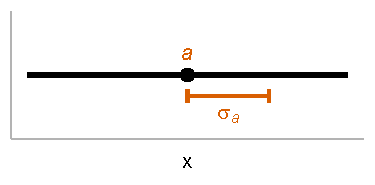
\includegraphics[width=1.2\columnwidth]{figs/2-mean_sd_interval.pdf}
  \end{minipage}

This is one approach taken by \textit{Vega-lite}: it provides an \texttt{errorbar}\footnote{\label{foot:errorbar}\texttt{errorbar} is, in my view, a misnomer, as is \texttt{xError}: fundamentally, the mark calculates a Gaussian interval, which might be for a distribution being used to represent error in an estimate, but might not. \textit{Error} is not the generic notion at play; a standard deviation is; and the generic mark is an interval, not an error bar.} mark (analogous to \textit{pointinterval}) and an \texttt{xError}  channel (analogous to $x_\textsc{sd}$). I'll refer to this notation as the $\{x, x_\textsc{sd}\}$ approach.

The problem, fundamentally, is that not all uncertainty is well-represented by a Gaussian distribution. Consider uncertainty in a proportion (bounded at 0 and 1, thus as estimates approach the boundary the interval becomes asymmetric---yet Gaussian intervals must be symmetric) or uncertainty in a variance parameter (bounded below at 0). Or, consider the ubiquitous Student-\textit{t} confidence interval: as the degrees of freedom go to $\infty$, a Student-\textit{t} distribution is well-approximated by the Normal, but with low degrees of freedom (incidentally common in small-\textit{n} studies---like at \textsc{vis}), the tails of the distribution become fatter, and the Normal distribution is a poor approximation. Thus, a more general approach is needed.

The obvious alternative, at least for interval representations, is to simply specify the endpoints of the intervals; e.g. for a 95\% Gaussian interval:

\noindent
\begin{minipage}{.5\columnwidth}
\begin{align*}
\mu &\rightarrow x\\
\mu - 1.96 \cdot \sigma &\rightarrow x_\textsc{min}\\
\mu + 1.96 \cdot \sigma &\rightarrow x_\textsc{max}\\
\textsc{geom} &= \mathit{pointinterval}
\end{align*}
  \end{minipage}%
  \begin{minipage}{.4\columnwidth}
    \centering
    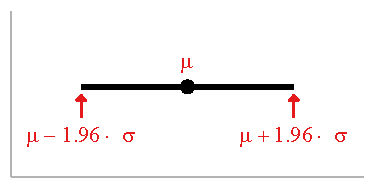
\includegraphics[width=1.2\columnwidth]{figs/2-xmin_xmax_interval.pdf}
  \end{minipage}
\hfill\break

Here, the magic values $-1.96$ and $+1.96$ are the $(1-95\%/2) = 2.5\%$th and $(1+95\%/2) = 97.5\%$th quantiles of the standard Normal distribution, thus yielding a $97.5\% - 2.5\% = 95\%$ interval. This is generic in the sense that any interval can be represented, but unsatisfying in the sense that we seem to have lost some level of abstraction that was present when we were just thinking in terms of estimates and their variances. This approach also requires that the user knows how to make these calculations. Both \textit{ggplot2} (with \texttt{geom\_pointrange}) and \textit{Vega-lite} (with the \texttt{x} and \texttt{x2} channels supplied to \texttt{errorbar}) offer a variant of this solution for pre-calculated intervals. 

I will offer a different solution: to instead represent intervals as properties of a distribution, allowing us to neatly handle both the simple case of Gaussian error and more complex cases. Centering distributions---not standard deviations or intervals---in the specification of uncertainty will also allow us to build a richer set of uncertainty representations.

\section{Uncertainty visualization as\\distributional visualization}

\subsection{Intervals}

Imagine we represent an uncertain value generically as a distribution, or a random variable, $M$. Importantly, I do not consider this a \textit{probability} distribution necessarily: it could be a probability distribution, but it could also be a \textit{confidence} distribution, which is a frequentist generalization of sampling distributions and bootstrap distributions~\cite{xie2013confidence}. Its defining characteristic will be that it has a cumulative distribution function (\textsc{cdf}), $F_M(x)$, which is:
\begin{itemize}
    \item For a probability distribution, $F_M(x) = \Pr(M \le x)$, the probability that $M$ is less than or equal to $x$.
    \item   For a confidence distribution, $F_M(x) = \gamma$  is the confidence $\gamma$ at which $x$ would be the upper limit of a one-sided $\gamma\%$ confidence interval, $[-\infty, x]$, for $M$. That sentence is pretty typical of convoluted frequentist definitions, so it might be easier to think in terms of the inverse: $F_M^{-1}(\gamma)$ yields the value $x$, which is the upper limit of a one-sided $\gamma\%$ confidence interval on $M$: $[-\infty,x]$. So $[-\infty, F_A^{-1}(0.95)]$ is a one-sided 95\% confidence interval on $M$.
\end{itemize}

For either representation, we may also be interested in other functions of the distribution. These include the derivative of the cumulative distribution function, i.e. the density function (or the mass function, if the distribution is discrete), $f_M(x)$, as well as the inverse of the \textsc{cdf} (also known as the quantile function), $F_M^{-1}(x)$. Given these functions, we can generate a variety of uncertainty representations, including but not limited to density plots and intervals.

For example, a median and $\gamma\%$ quantile interval could be defined generically on any distribution $M$ as follows:

\noindent
\begin{minipage}{.5\columnwidth}
\begin{align*}
\operatorname{median}(M) &\rightarrow x\\
F_M^{-1}\left[\frac{1 - \gamma}{2}\right] &\rightarrow x_\textsc{min}\\
F_M^{-1}\left[\frac{1 + \gamma}{2}\right] &\rightarrow x_\textsc{max}\\
\textsc{geom} &= \mathit{pointinterval}
\end{align*}
\end{minipage}%
  \begin{minipage}{.4\columnwidth}
    \centering
    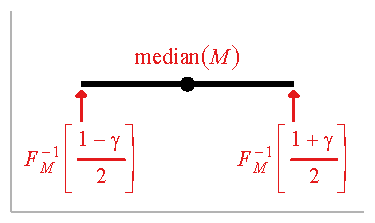
\includegraphics[width=1.2\columnwidth]{figs/3-geom_pointinterval_quantiles.pdf}
  \end{minipage}
\hfill\break

If $M$ is a probability distribution, this is a Bayesian \textit{credible }interval, and if $M$ is a confidence distribution, this is a frequentist \textit{confidence} interval. This lets us abstract over the petty battles between this or that statistical camp and get to the meaningful business of visualizing uncertainty. This also allows us something not present in other attempts so far: to make it easy to specific multiple interval sizes, and to map interval size itself onto an aesthetic. For example, if we\footnote{Yes yes, I am using both ``I'' and ``we'' in this paper. ``I'' is me, and ``we'' is the conspiratorial ``we'': I'd like to hope you'll come along with me on this exciting journey of trying to sort out reasonable ways to visualize uncertainty.} wanted to show two intervals, a 95\% and a 66\%, where the smaller interval is shown as a thicker line, we could write:

\noindent
\begin{minipage}{.5\columnwidth}

\begin{align*}
\operatorname{median}(M) &\rightarrow x\\
F_M^{-1}\left[\frac{1 - \gamma}{2}\right] &\rightarrow x_\textsc{min}\\
F_M^{-1}\left[\frac{1 + \gamma}{2}\right] &\rightarrow x_\textsc{max}\\
\gamma &\rightarrow \mathit{linewidth}\\
\textsc{geom} &= \mathit{pointinterval}\\
\gamma &\in \{0.66, 0.95\}
\end{align*}
\end{minipage}%
  \begin{minipage}{.4\columnwidth}
    \centering
    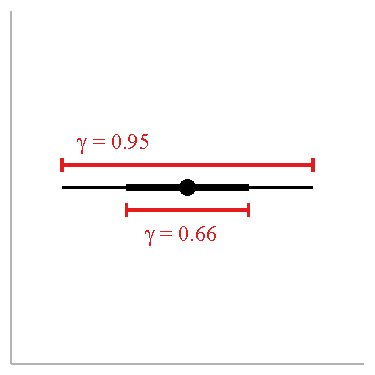
\includegraphics[width=1.2\columnwidth]{figs/3-stat_pointinterval_linewidth.pdf}
  \end{minipage}
\hfill\break

This is a not-uncommon approach that tries to avoid dichotomous thinking by showing multiple intervals of different masses. It also has the nice grammar-of-graphics-ish property of mapping the mass ($\gamma$) onto the width of the line, instead of creating two explicit, separate layers, each specifying a different interval---it makes the mass into \textit{data}.\footnote{I learned at least two useful things from a relational databases class in undergrad: (1) it's always better to put data into rows than into column names of tables---an insight that stems from database \textit{normal forms}~\cite{codd1990relational} (distinctions between which I have long forgotten) or what some statisticians call \textit{tidy data}~\cite{hadley2014tidy}; and (2) you are rarely at Google scale, so you're probably better off with a relational database with proper transactions than some dumb old key value store. The latter lesson each of my students refuses to learn until they build a webapp to collect data from 300 people using some newfangled database they aren't the target users for, and end up with garbage. Kids these days, etc.}\footnote{Students of the grammar of graphics will note that I've left off details of the scale functions here (and elsewhere). In this case, the $linewidth$ mapping and scale function will need to include conversion to an ordinal data type (\texttt{ordered} in R). This is mostly too minor a concern for the high level at which I want to keep notational discussion in this paper, though there is an example in \cref{sec:dotplots} where we'll have to get into it.} This also makes it easy to generalize to other visualizations, e.g. by modifying the previous specification to map mass onto \textit{color} instead of \textit{linewidth}:


\noindent
\begin{minipage}{.5\columnwidth}

\begin{align*}
\gamma &\rightarrow \mathit{color}\\
\textsc{geom} &= \mathit{pointinterval}\\
\gamma &\in \{0.50, 0.80, 0.95\}
\end{align*}
\end{minipage}%
  \begin{minipage}{.4\columnwidth}
    \centering
    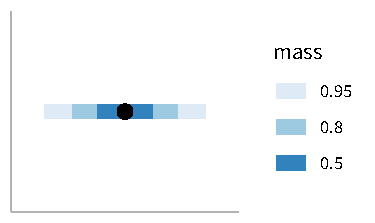
\includegraphics[width=1.2\columnwidth]{figs/3-stat_pointinterval_color.pdf}
  \end{minipage}
\hfill\break


On the other hand, these are still a bit low-level: they require the user to know how to calculate interval endpoints from the quantile function. This also limits us specifically to quantile intervals, when other intervals types, such as highest-density intervals~\cite{hyndman1996computing} and shortest intervals~\cite{liu2015spi}, might be preferable. Thus, \textit{ggdist} also supplies a \textit{stat} version of \textit{pointinterval}, which bundles up some statistical calculations and default aesthetic mappings with the \textit{pointinterval} geometry. All \textit{stat}s in \textit{ggdist} support the $x_\textsc{dist}$ and $y_\textsc{dist}$ aesthetics, onto which objects that represent distributions can be mapped. They also allow the user to specify the type of point and interval used, and generate the corresponding values and mappings for $x$, $x_\textsc{min}$, $x_\textsc{max}$, and \textit{linewidth}. This changes the specification to something like:


\noindent
\begin{minipage}{.5\columnwidth}

\begin{align*}
M &\rightarrow x_\textsc{dist}\\
\textsc{stat} &= \mathit{pointinterval}\\
\textsc{point} &= \mathit{median}\\
\textsc{interval} &= \textit{quantile interval}\\
\gamma &\in \{0.66, 0.95\}
\end{align*}
\end{minipage}%
  \begin{minipage}{.4\columnwidth}
    \centering
    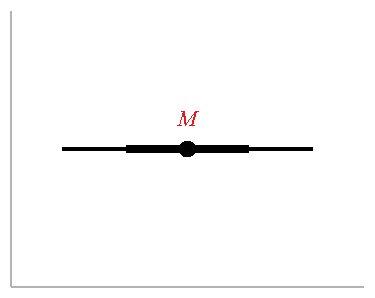
\includegraphics[width=1.2\columnwidth]{figs/3-stat_pointinterval_A.pdf}
  \end{minipage}
\hfill\break

The representation of the distribution $M$ could be a sample-based representation, e.g. a bunch of draws from a Bayesian posterior or from a bootstrap distribution, or it could be an object representing a theoretical distribution in terms of its parameters, such as a Normal distribution with a defined mean and standard deviation. Point estimates and interval types can be defined by arbitrary functions of distributions, and predefined functions for mean, median, and mode, and quantile, highest-density, and shortest intervals are provided. This generalizes the $\{x, x_\textsc{sd}\}$ approach used by \textit{Vega-lite} to any distribution type while abstracting over the specifics of how point estimates and intervals are calculated.

In implementation, \textit{ggdist} allows distributions to be represented by numeric vectors (a sample-based representation), objects from the \textit{distributional } R package~\cite{oharawild2022distributional} (which supports theoretical distributions), and \texttt{rvar} objects from the \textit{posterior} R package~\cite{burkner2022posterior} (a sample-based representation that mimics numeric arrays in R). For example, if we re-create the $\{x, x_\textsc{sd}\}$ representation abstractly thus:

\noindent
\begin{minipage}{.5\columnwidth}

\begin{align*}
\operatorname{Normal}(\mu, \sigma) &\rightarrow x_\textsc{dist}\\
\textsc{stat} &= \mathit{pointinterval}\\
\textsc{point} &= \mathit{median}\\
\textsc{interval} &= \textit{quantile interval}\\
\gamma &\in \{0.66, 0.95\}
\end{align*}
\end{minipage}%
  \begin{minipage}{.4\columnwidth}
    \centering
    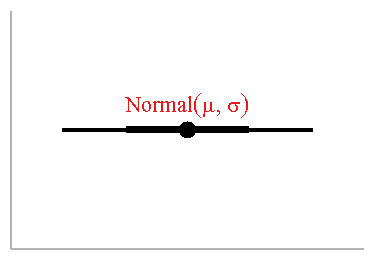
\includegraphics[width=1.2\columnwidth]{figs/3-stat_pointinterval_normal.pdf}
  \end{minipage}
\hfill\break

In \textit{ggdist}, using \texttt{distributional::dist\_normal}, the specification is quite similar:

\begin{centerverbatim}
ggplot(data) +
  aes(xdist = dist_normal(mu, sigma)) +
  stat_pointinterval(
    point_interval = median_qi, 
    .width = c(.66, .95)
  )
\end{centerverbatim}

These happen to be the default values for \texttt{point\_interval} and \texttt{.width} ($\gamma$),\footnote{For historical reasons that have to do with a combination of a very long discussion with a bunch of people on the Stan probabilistic programming language forums~\cite{kay2018stannames} and naming conventions in some R \textsc{api}s for fixed arguments to functions with variable argument lists~\cite{tidyverse2020dotprefix}, $\gamma$ in \textit{ggdist} is spelled \texttt{.width}. Reflecting on my past mistakes, a better name would be  \texttt{mass}.} so just \texttt{stat\_pointinterval()}  also works here. To demonstrate generalizing this approach, consider the very common need of placing uncertainty intervals on the results of a $t$-test, which can be derived from a $t_\nu(\mu, \sigma)$  distribution with $\nu$ degrees of freedom, location $\mu$ (e.g. an estimated mean), and scale $\sigma$ (e.g. a standard error). Given these three numbers in a data frame, a visualization specification might be:

\noindent
\begin{minipage}{.5\columnwidth}

\begin{align*}
t_{\nu}(\mu, \sigma) &\rightarrow x_\textsc{dist}\\
\textsc{stat} &= \mathit{pointinterval}
\end{align*}
\end{minipage}%
  \begin{minipage}{.4\columnwidth}
    \centering
    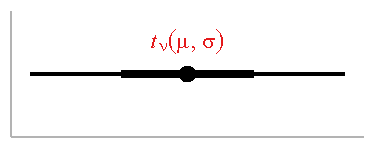
\includegraphics[width=1.2\columnwidth]{figs/3-stat_pointinterval_student_t.pdf}
  \end{minipage}
\hfill\break


Which in \textit{ggdist} is:

\begin{centerverbatim}
ggplot(data) +
  aes(xdist = dist_student_t(nu, mu, sigma)) +
  stat_pointinterval()
\end{centerverbatim}

Thus the code matches up closely to the abstract notation.

\subsection{Ribbons}

Once we have \textit{pointinterval} representations, it is straightforward to develop uncertainty band representations by generalizing points to lines and intervals to ribbons---thus, \textit{lineribbon}. Imagine a regression that models car miles per gallon based on weight (the details of the function $g$ are not important):

\[
\log(\mathit{mpg}) \sim \operatorname{Normal}\left(g(\mathit{weight}), \sigma\right)
\]
Such a model could provide a predictive distribution for a car's miles per gallon conditional on its weight: $p(\mathit{mpg} \mid \mathit{weight})$, which we might want to plot alongside the raw data. If a \textit{lineribbon} is a geometry combining a line with an arbitrary number of uncertainty bands around it, abstractly, we want something like this:

\noindent
\begin{minipage}{.5\columnwidth}

\begin{align*}
\mathit{weight} &\rightarrow x\\
p(\mathit{mpg} \mid \mathit{weight}) &\rightarrow y_\textsc{dist}\\
\gamma &\rightarrow \mathit{fill}\\
\textsc{stat} &= \mathit{lineribbon}\\
\gamma &\in \{0.50, 0.80, 0.95\}
\end{align*}
\end{minipage}%
  \begin{minipage}{.4\columnwidth}
    \centering
    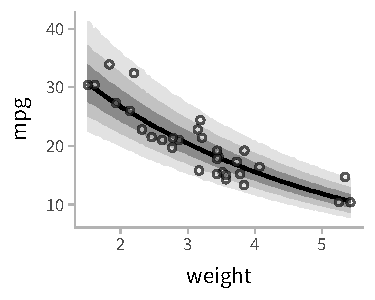
\includegraphics[width=1.2\columnwidth]{figs/3-lineribbon.pdf}
  \end{minipage}
\hfill\break


I include the raw data as a separate \textit{point} geometry layer as well, for comparison. Assuming \texttt{fit}  is a Bayesian version of such a model fit using the \textit{brms} modeling package in R, and \texttt{preds} is a data frame of desired \textit{weight} values to predict on, we can add a column to \texttt{preds} that contains a random variable representation of $p(\mathit{mpg} \mid \mathit{weight})$ using \texttt{brms::posterior\_predict}~\cite{burkner2018brms} and the \texttt{posterior::rvar}  data type~\cite{burkner2022posterior}. The latter is a data type I created\footnote{This was a slightly insane idea in itself, given the way that base R data types work. As R's classes work based on generic \textit{functions}, rather than classes with a well-defined set of methods, this requires tracking down all the various functions implemented to work with arrays and vectors in the language and providing implementations for them for random variable arrays. Indexing functions especially are annoying, as there are half a dozen different ways to index into R arrays, each with myriad corner cases. Anyway.} specifically to wrap large samples that represent distributions into objects that mimic R vectors and arrays, and which can be added to data frames:

\begin{centerverbatim}
preds = preds |> mutate(
  mpg_given_weight = rvar(posterior_predict(fit, preds)
)
\end{centerverbatim}

Given this data frame, the equivalent of the abstract specification above is:

\begin{centerverbatim}
ggplot(preds) +
  aes(x = weight, ydist = mpg_given_weight) +
  stat_lineribbon()
\end{centerverbatim}

\texttt{stat\_lineribbon} defaults to \texttt{.width = c(.5, .8, .95)} and maps the resulting \texttt{.width} onto the \texttt{fill} aesthetic, so we do not need to specify \texttt{.width} or the \texttt{fill} mapping for this example. Once we have a multiple-ribbon geometry, it is easy to create other uncertainty visualization types, like gradient fan charts~\cite{bowman2019graphics,jackson2008displaying}. For example, we could use a large number of intervals, say $k = 50$ or $100$, with masses between 0 and 1 (exclusive):

\noindent
\begin{minipage}{.5\columnwidth}

\begin{align*}
\gamma &\rightarrow \mathit{fill}\\
\textsc{stat} &= \mathit{lineribbon}\\
\gamma &\in \left\{\frac{i - 0.5}{k} \mathrel{}\middle|\mathrel{} i \in 1 \dots k \right\}\\
k &= 100
\end{align*}
\end{minipage}%
  \begin{minipage}{.4\columnwidth}
    \centering
    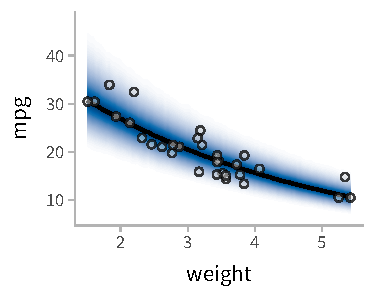
\includegraphics[width=1.2\columnwidth]{figs/3-lineribbon_fan.pdf}
  \end{minipage}
\hfill\break


This set of $k$  $\gamma$ values is the same sequence generated by the \texttt{ppoints(k)} function in R, so we can pass \texttt{.width = ppoints(100)} to \texttt{stat\_lineribbon} to get a gradient fan chart with 100 intervals. This stems directly from the choice to make $\gamma$ into data that can be mapped onto aesthetics, and is one example of support for a chart type that was a happy accident of \textit{ggdist}'s design.\footnote{This happy accident was discovered in my response to user's question in \textit{tidybayes} \href{https://github.com/mjskay/tidybayes/issues/103}{issue \#103}.}

\subsection{Slabs}

Speaking of gradients, the obvious other direction to go for uncertainty---if we are to move beyond intervals---is density plots. Most grammar of graphics implementations support density plots, but these are typically designed only for sample-based representations: they calculate a kernel density estimate (\textsc{kde}) from a sample and allow this to be visualized. Given \textit{ggdist}'s core abstraction of distributions, we can take this a step further, visualizing both sample-based representations and theoretical distributions.\footnote{\label{foot:jacobians}You may be tempted to say: but Matthew, of course you could easily pre-calculate densities from a theoretical density function and plot them, e.g. using \texttt{ggplot2::stat\_function}. Unfortunately, once you add non-linear axis transformation into the mix, this is a recipe for silent errors caused by failing to adjust the density by the derivative of the transformation---an error \textit{ggdist} prevents. See \cref{sec:jacobians}.} 

However, stopping at \textit{just} densities seems the wrong level of abstraction:\footnote{See earlier footnote\textsuperscript{\ref{foot:errorbar}} about \textit{error bars} versus \textit{intervals}.} many useful uncertainty visualizations can be created through the whole suite of distributional functions: \textsc{cdf}s, densities, and quantiles. Thus, \textit{ggdist} instead has a notion of a \textit{slab} geometry, which has a \textit{thickness} onto which arbitrary functions of the distribution can be mapped. For example, imagine two \textit{group}s, \textit{a} and \textit{b}, each with uncertainty in its mean represented by a random variable $M \mid group$. We could specify a density plot of these distributions as:

\noindent
\begin{minipage}{.5\columnwidth}

\begin{align*}
M &\rightarrow x_\textsc{dist}\\
\textit{group} &\rightarrow y\\
f_M(x) &\rightarrow \textit{thickness}\\
\textsc{stat} &= \mathit{slab}
\end{align*}
\end{minipage}%
  \begin{minipage}{.4\columnwidth}
    \centering
    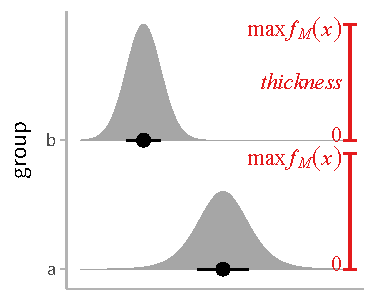
\includegraphics[width=1.2\columnwidth]{figs/3-slab_density_two_groups.pdf}
  \end{minipage}
\hfill\break

I also include a \textit{pointinterval} with a median and 66\% interval above (and elsewhere in this section) for reference. The \textit{slab}s have a subscale for \textit{thickness},\footnote{Grammar of graphics aficionados might ask: why not use faceting instead of creating a new positional subscale? Experience has shown many situations where faceting doesn't cut it: for example, when displaying many related estimates at once within a single group, people often group together geometries and then \textit{dodge} them; a \textit{thickness} subscale supports this usage but facets do not.} which is an orientation-aware aesthetic (if the distributions were mapped onto $y_\textsc{dist}$, \textit{thickness} would act as a width instead of height), with a fixed baseline: values of 0 on the thickness scale always correspond to the base of the slab. This makes it appropriate for both probability densities and $\textsc{cdf}$s, both of which have a natural 0 point. In the above example, the density $f_M(x)$ is mapped onto \textit{thickness}, creating a traditional density plot. Importantly, because the geometries use the same scale, both subscales have the same overall maximum \textit{thickness}, which ensures that the area under both densities is equal.\footnote{This default is, most of the time, what you want, as it preserves the property that each distribution integrates to 1. For exceptions to this rule, \textit{ggdist} provides a \texttt{normalize} option and a \texttt{scale\_thickness\_shared} function which allow finer control over how thickness scales are shared across groups, panels, and geometries.} 

This is the default output of \texttt{stat\_slab()} in \textit{ggdist}, which maps densities onto the \textit{thickness} aesthetic. If desired, the mapping $f_M(x) \rightarrow \textit{thickness}$ can be translated to code in one of two ways:

\begin{enumerate}
    \item \texttt{aes(thickness = after\_stat(pdf))}: This says to map the \texttt{pdf} \textit{computed variable} onto \textit{thickness}. Computed variables in \textit{ggplot2} are calculated by \textit{stat}s and made accessible in aesthetic mappings by wrapping the mapping specification in \texttt{after\_stat()}. \textit{ggdist} stats provide several computed variables, including \texttt{pdf}, \texttt{cdf}, and \texttt{.width}.
    \item \texttt{aes(thickness = !!p\_(x))}:  This uses a small domain-specific language for probability expressions I added to \textit{ggdist}, and is intended to more closely mimic a mapping like $p(x) \rightarrow thickness$ in code. The \texttt{!!} pseudo-operator comes from the \textit{rlang} meta-programming R package, and performs \textit{unquotation}~\cite{wickham2019advanced}: it inserts the expression returned by \texttt{p\_(x)}, which in this case is \texttt{after\_stat(pdf)}, into the \texttt{aes} call.\footnote{I added this syntax relatively recently, when \textit{ggplot2} deprecated \texttt{stat()}, which used to be a synonym for \texttt{after\_stat()}. This (1) made expressions with \texttt{after\_stat} needlessly verbose and (2) replaced a declarative verb, \texttt{stat}---which indicates the type of expression at play but not when it is computed---with a procedural verb, \texttt{after\_stat}. I feel that this name change violates the declarative foundations of \textit{ggplot2}, and the mini-\textsc{dsl} for probabilistic expressions in \textit{ggdist} is my small protest against it.}
\end{enumerate}

Slab geometries have several useful properties which help make them useful for creating a variety of uncertainty visualizations. One important property is that the \textit{alpha} (opacity), \textit{fill}, and outline \textit{color} aesthetics of the slabs can have data values mapped onto them at a sub-geometry level.\footnote{Just as an implementation note, this happens to be an incredible pain in the ass. Prior to R 4.1, the R graphics engine did not have proper gradient support, so this involved manually sub-dividing geometries and interpolating thickness values at cutpoints between contiguous blocks of color. Now, with proper gradient support in some R graphics output formats (e.g. \textsc{svg} and \textsc{pdf}), \textit{ggdist} can output high-quality color gradients, and as of this writing is one of the only R packages to do so (even base \textit{ggplot2} has not implemented it yet).} This functionality, combined with the ability to map arbitrary distribution functions, means we can easily recreate a bunch of visualizations from the literature. The obvious first example would be a color gradient plot~\cite{jackson2008displaying}, by mapping density onto \textit{alpha}:


\noindent
\begin{minipage}{.5\columnwidth}

\begin{align*}
M &\rightarrow x_\textsc{dist}\\
\textit{group} &\rightarrow y\\
f_M(x) &\rightarrow \textit{alpha}\\
\textsc{stat} &= \mathit{slab}
\end{align*}
\end{minipage}%
  \begin{minipage}{.4\columnwidth}
    \centering
    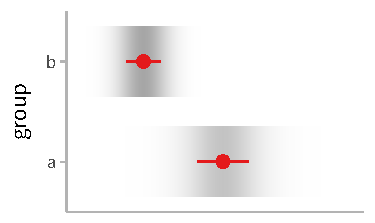
\includegraphics[width=1.2\columnwidth]{figs/3-slab_gradient_two_groups.pdf}
  \end{minipage}
\hfill\break

This translates naturally to \texttt{aes(alpha = !!p\_(x))}. Fine fine, but let's get \textit{weird}. Back in 2014, the inimitable Michaels Correll and Gleicher---arguing that error bars should be considered harmful~\cite{correll2014error}---proposed instead a visualization which has a solid bar inside the 95\% interval and gradient tails that fade out beyond the interval, to emphasize the arbitrariness of the 95\% confidence level. We can use the \textsc{cdf} to construct a function with these properties, and map it to \textit{alpha}:

\noindent
\begin{minipage}{.5\columnwidth}

\begin{align*}
-\max \left[ \begin{matrix} \lvert 2 F_M(x) - 1 \rvert \\ 0.95 \end{matrix} \right] &\rightarrow \textit{alpha}\\
\textsc{stat} &= \mathit{slab}
\end{align*}
\end{minipage}%
  \begin{minipage}{.4\columnwidth}
    \centering
    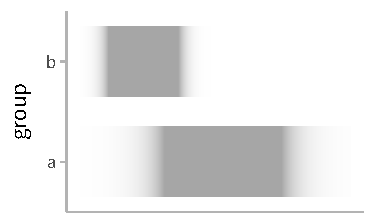
\includegraphics[width=1.2\columnwidth]{figs/3-slab_gradient_correll.pdf}
  \end{minipage}
\hfill\break

In \textit{ggdist} this function is either:
\begin{itemize}
    \item \texttt{-pmax(abs(2*after\_stat(cdf) - 1), .95)} or
    \item    \texttt{-pmax(abs(2*!!Pr\_(X <= x) - 1), .95)}, using the probability expression mini-\textsc{dsl}.
\end{itemize}

Thus, \textit{ggdist} can create this particularly weird uncertainty visualization without breaking the bonds of its core abstraction. Importantly, the function I've used to construct the tails is not arbitrary; it is meaningful in itself: $1 - \lvert 2 F_M(x) - 1 \rvert$ is the \textit{consonance curve}~\cite{amrhein2022discuss}, which (in the frequentist interpretation) is the two-sided \textit{p}-value for the null hypothesis \textit{x}. Horizontal slices through this curve at a height of $\alpha$ are $(1 - \alpha)\%$ quantile confidence intervals:


\noindent
\begin{minipage}{.5\columnwidth}

\begin{align*}
1 - \lvert 2 F_M(x) - 1 \rvert &\rightarrow \textit{thickness}\\
\textsc{stat} &= \mathit{slab}
\end{align*}
\end{minipage}%
  \begin{minipage}{.4\columnwidth}
    \centering
    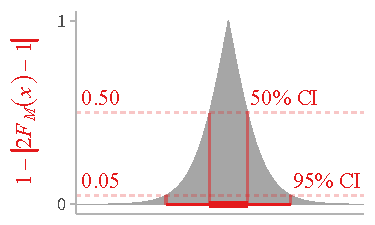
\includegraphics[width=1.2\columnwidth]{figs/3-slab_consonance.pdf}
  \end{minipage}
\hfill\break

Fair enough, but let's get \textit{weirder}: in 2021, Helske et al~\cite{helske2021can}, inspired by Correll and Gleicher, proposed combining their gradient tail with a violin plot. We can do that by adding back in the density-to-thickness mapping, and use the \textsc{side} parameter, which specifies if the slab should be drawn on the \textit{top} side (default), \textit{bottom} side, or \textit{both}. I'll also adjust the tails to fade outside the 85\% interval, since otherwise the fading is hard to see in the skinny tails of the violin:

 \noindent
\begin{minipage}{.5\columnwidth}

\begin{align*}
f_M(x) &\rightarrow \textit{thickness}\\
-\max \left[ \begin{matrix} \lvert 2 F_M(x) - 1 \rvert \\ 0.85 \end{matrix} \right] &\rightarrow \textit{alpha}\\
\textsc{stat} &= \mathit{slab}\\
\textsc{side} &= \mathit{both}
\end{align*}
\end{minipage}%
  \begin{minipage}{.4\columnwidth}
    \centering
    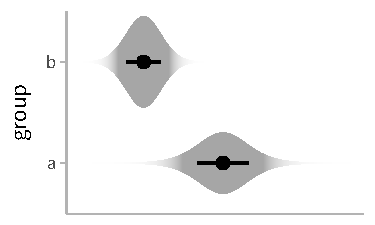
\includegraphics[width=1.2\columnwidth]{figs/3-slab_violin_gradient.pdf}
  \end{minipage}
\hfill\break

Okay fine, but let's get \textit{even weirder}: Helske et al~\cite{helske2021can} further suggested using discrete intervals for the colors instead of a gradient, to aid discriminability. We can do that too! A key feature of the \textit{slab} stat is that it \textit{also} computes intervals, and for each point along the slab, retains a column indicating the mass ($\gamma$) of the smallest requested interval containing that point.\footnote{This can also be done by discretizing the \textsc{cdf}, and that was the recommended approach in earlier versions of \textit{ggdist}; see the \href{https://mjskay.github.io/ggdist/reference/cut_cdf_qi.html}{\texttt{cut\_cdf\_qi} function}. However, that does not generalize to other kinds of intervals, like highest-density intervals---hence the approach described here.}  This means that we can integrate intervals directly into the slab by mapping $\gamma$ onto \textit{alpha} or \textit{fill}:


 \noindent
\begin{minipage}{.5\columnwidth}

\begin{align*}
f_M(x) &\rightarrow \textit{thickness}\\
\gamma &\rightarrow \textit{fill}\\
\gamma &\in \{0.5, 0.8, 0.95, 1\}\\
\textsc{stat} &= \mathit{slab}\\
\textsc{side} &= \mathit{both}
\end{align*}
\end{minipage}%
  \begin{minipage}{.4\columnwidth}
    \centering
    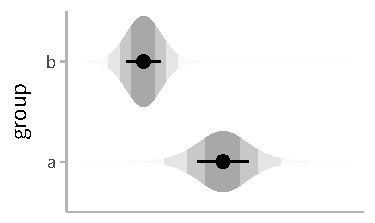
\includegraphics[width=1.2\columnwidth]{figs/3-slab_violin_interval.pdf}
  \end{minipage}
\hfill\break

Helske describes these violin-interval plots as ``more challenging to create''; \textit{ggdist} supports them naturally through a combination of its core features. This demonstrates the power of allowing distribution functions and intervals to be easily mapped to aesthetics within a single geometry.

Another variation on violin plots is the \textit{raindrop plot} of Barrowman and Myers~\cite{barrowman2003raindrop}, which maps log-density instead of density onto \textit{thickness} inside a desired interval, say 95\%:


 \noindent
\begin{minipage}{.5\columnwidth}

\begin{align*}
\arraycolsep=2.5pt \left.\begin{array}{ll} \log f_M(x) & \textrm{if } \gamma \le .95\\ \varnothing & \textrm{otherwise}\end{array}\right\} &\rightarrow \textit{thickness}\\
\textsc{stat} &= \mathit{slab}\\
\textsc{side} &= \mathit{both}
\end{align*}
\end{minipage}%
  \begin{minipage}{.4\columnwidth}
    \centering
    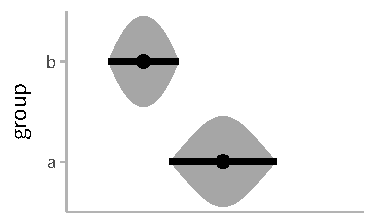
\includegraphics[width=1.2\columnwidth]{figs/3-slab_raindrop.pdf}
  \end{minipage}
\hfill\break

The rationale here is that some distributional features, such as fat tails (kurtosis), can be easier to see in log-density than density~\cite{barrowman2003raindrop}. In \textit{ggdist}, the above spec is written:

\begin{centerverbatim}
aes(thickness = ifelse(.width <= .95, log(!!p_(x)), NA)) +
stat_slab(side = "both", normalize = "groups")
\end{centerverbatim}

Where \texttt{normalize = "groups"} is needed to tell the slab to normalize thickness on a per-group basis, as log-density does not have a natural zero point. Without this, the endpoints of the arcs defining the ``raindrops'' may not reach the \textit{thickness} baseline.

Another interesting\footnote{\textsc{aka} weird.}\footnote{Yes, there are a lot of footnotes. No, I don't care.} uncertainty visualization from the literature is Haber and Wilkinson's~\cite{haber1982perceptual} \textit{fuzzygram}, i.e. \textit{fuzzy histogram}. We can generalize it to a \textit{fuzzy bar chart}. This chart type has what I would call a compelling \textit{generative story}: an explanation you can give for how the uncertainty encoding in the chart arises based on some generative process. Imagine we want to add uncertainty to a bar chart, and we have a distribution for the uncertainty in the value encoded in each bar. Now say we sample a large number of semi-transparent bar charts from these distributions, and overlay them all on top of each other. As the number of charts approaches $\infty$ and the opacity of any given chart goes to 0, the stack of overlapping bars for each value will begin to resemble the complementary \textsc{cdf}, $1 - F(x)$, of that distribution.\footnote{Assuming additive blending and opacities that sum to 1.} That insight leads to the following encoding:

 \noindent
\begin{minipage}{.5\columnwidth}

\begin{align*}
1 - F_M(x) &\rightarrow \textit{alpha}\\
\textsc{stat} &= \mathit{slab}
\end{align*}
\end{minipage}%
  \begin{minipage}{.4\columnwidth}
    \centering
    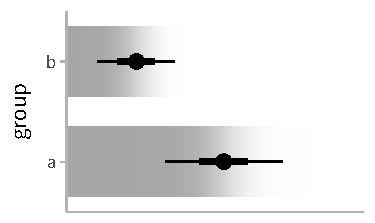
\includegraphics[width=1.2\columnwidth]{figs/3-slab_fuzzygram.pdf}
  \end{minipage}
\hfill\break

I would describe this chart type as theoretically interesting but interpretationally problematic. Anecdotally, without the overlaid reference point and interval, folks I show this to often do not correctly identify the mean of the distribution, believing the darker parts of the bar are more likely (a not unreasonable misinterpretation).\footnote{I don't know if this is an example of within-the-bar bias~\cite{newman2012bar} or not.} On the other hand, I do like the idea of \textit{generative stories} in uncertainty visualization; for example, I've used Plinko boards to \href{https://presidential-plinko.com/}{depict uncertainty in election forecasts}, which try to capitalize on a physical process---one that might intuitively\footnote{As this is an uncertainty visualization paper, I am professionally obligated to use ``intuitive'' at least once without defining it.} feel random to people---to depict uncertainty through a form of \textit{sedimentation}~\cite{huron2013sediment}.

Another advantage to being able to map arbitrary data values onto slab aesthetics is that we can map the results of logical conditions onto those aesthetics. A common procedure in the Bayesian estimation community is to use regions of practical equivalence (\textsc{rope}s)~\cite{kruschke2018rejecting}. Say, for example, you are interested in whether an estimate is ``practically'' equal to 0; you would define a \textsc{rope} around 0 of $\pm$ some small effect size within which you would consider the value so close to 0 it is effectively indistinguishable from it. Then you can ask: \textit{what is the probability the value is practically equivalent to 0?} We can visualize this probability by highlighting the \textsc{rope} on a density:

\noindent
\begin{minipage}{.5\columnwidth}

\begin{align*}
f_M(x) &\rightarrow \textit{thickness}\\
\lvert x \rvert < 2 &\rightarrow \textit{fill}\\
\textsc{stat} &= \mathit{slab}
\end{align*}
\end{minipage}%
  \begin{minipage}{.4\columnwidth}
    \centering
    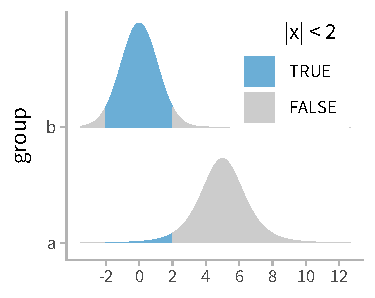
\includegraphics[width=1.2\columnwidth]{figs/3-slab_rope.pdf}
  \end{minipage}
\hfill\break

Here, $\Pr(\lvert x \rvert < 2)$---the probability the value is in a \textsc{rope} of $\pm2$---is directly encoded by the proportion of the area under the curve highlighted in blue. In \textit{ggplot2}, logical conditions can be mapped directly onto aesthetics, so in \textit{ggdist}, we can use \texttt{aes(fill = after\_stat(abs(x) < 2))} to create the above chart.

\subsection{Dotplots}
\label{sec:dotplots}

These days, when every other uncertainty visualization paper is about \textit{frequency framing} or \textit{discrete outcome} representations---spaghetti plots~\cite{cox2013visualizing,liu2018visualizing} hypothetical outcome plots~\cite{hullman2015hypothetical,kale2018hypothetical}, quantile dotplots~\cite{kay2016ish,fernandes2018uncertainty} and so on---I would be remiss to write a whole uncertainty visualization toolkit that can't make one measly discrete outcome visualization.\footnote{Plus, it would be a little silly of me to develop a whole-ass visualization toolkit that can't at least make quantile dotplots, since I came up with them in the first place~\cite{kay2016ish}.} The natural counterpart to the continuous encoding of the \textit{slab} geometry is \textit{ggdist}'s \textit{dots} geometry, which is designed to create Wilkinson dotplots~\cite{wilkinson1999dot} (on raw data)\footnote{And minor variations thereof, like \textit{beeswarm} plots, which can be created by setting $\textsc{side} = \textit{both}$ and (optionally) adjusting the \textsc{layout} parameter; see the \href{https://mjskay.github.io/ggdist/articles/dotsinterval.html}{\textit{dotsinterval} vignette} for examples.} and quantile dotplots.

Quantile dotplots were designed for uncertainty communication, and depict quantiles of a continuous distribution using a dotplot, to help the viewer reason about that distribution as a set of discrete possible outcomes~\cite{kay2016ish}. Put another way, they discretize the density function, and allow reasoning about intervals through counting: e.g., in a 100-dot quantile dotplot, $\Pr(X < 2)$ translates to the question, \textit{how many dots out of 100 are less than 2?} Continuing our example from the \textit{slab} geometries, here are two quantile dotplots using 100 dots each:

\noindent
\begin{minipage}{.5\columnwidth}

\begin{align*}
M &\rightarrow x_\textsc{dist}\\
\textit{group} &\rightarrow y\\
\textsc{stat} &= \mathit{dots}\\
\textsc{quantiles} &= 100
\end{align*}
\end{minipage}%
  \begin{minipage}{.4\columnwidth}
    \centering
    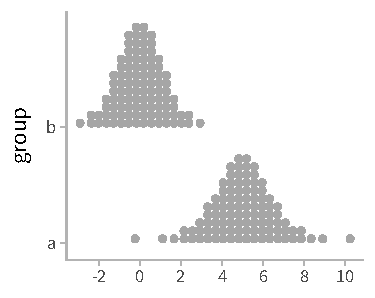
\includegraphics[width=1.2\columnwidth]{figs/3-dots_two.pdf}
  \end{minipage}
\hfill\break

It is worth noting that \textit{ggplot2} has a \textit{dotplot} geometry already, but that it is often awkward to use: as it uses a bin width specified by the user, there is no guarantee the dotplot fits inside the available space, often leading to dots running outside the plot region. By contrast, the \textit{dots} geometry in \textit{ggdist} uses numerical optimization to automatically find a shared bin width across all dotplots in the geometry that ensures they fit in the available space (notice I did not specify bin width above).\footnote{It also allows constraints on minimum and maximum bin width, and has various options for what to do if those constraints may be exceeded, such as compressing the layout so that dots may overlap. Anecdotally, automatic dotplot layout is one of the most popular features of \textit{ggdist}, as it relieves the intense frustration of the endless tweaking cycle to get the dot size right.}

One property of dotplots is the opportunity to encode additional information in the dots themselves. For example, we could take advantage of Unicode support in the \textit{shape} aesthetic (which determines how points are drawn) to use emoji to encode just how we feel about possible effect sizes in a distribution:\footnote{This example was inspired by \href{https://twitter.com/Birdbassador/status/916332327696875520}{a tweet} from Michael Correll suggesting effect sizes at \textsc{vis} might be best described with a dotplot of poop emojis. I was delighted to find that \textit{ggdist} \href{https://twitter.com/mjskay/status/1361366253424832512}{could replicate it}, but have spared the literature a faithful rendering of the poopmoji plot by opting for smiley faces here.}


\noindent
\begin{minipage}{.5\columnwidth}

\begin{align*}
M &\rightarrow x_\textsc{dist}\\
x > 0 &\rightarrow \textit{shape}\\
\textsc{stat} &= \mathit{dots}\\
\textsc{quantiles} &= 50
\end{align*}
\end{minipage}%
  \begin{minipage}{.4\columnwidth}
    \centering
    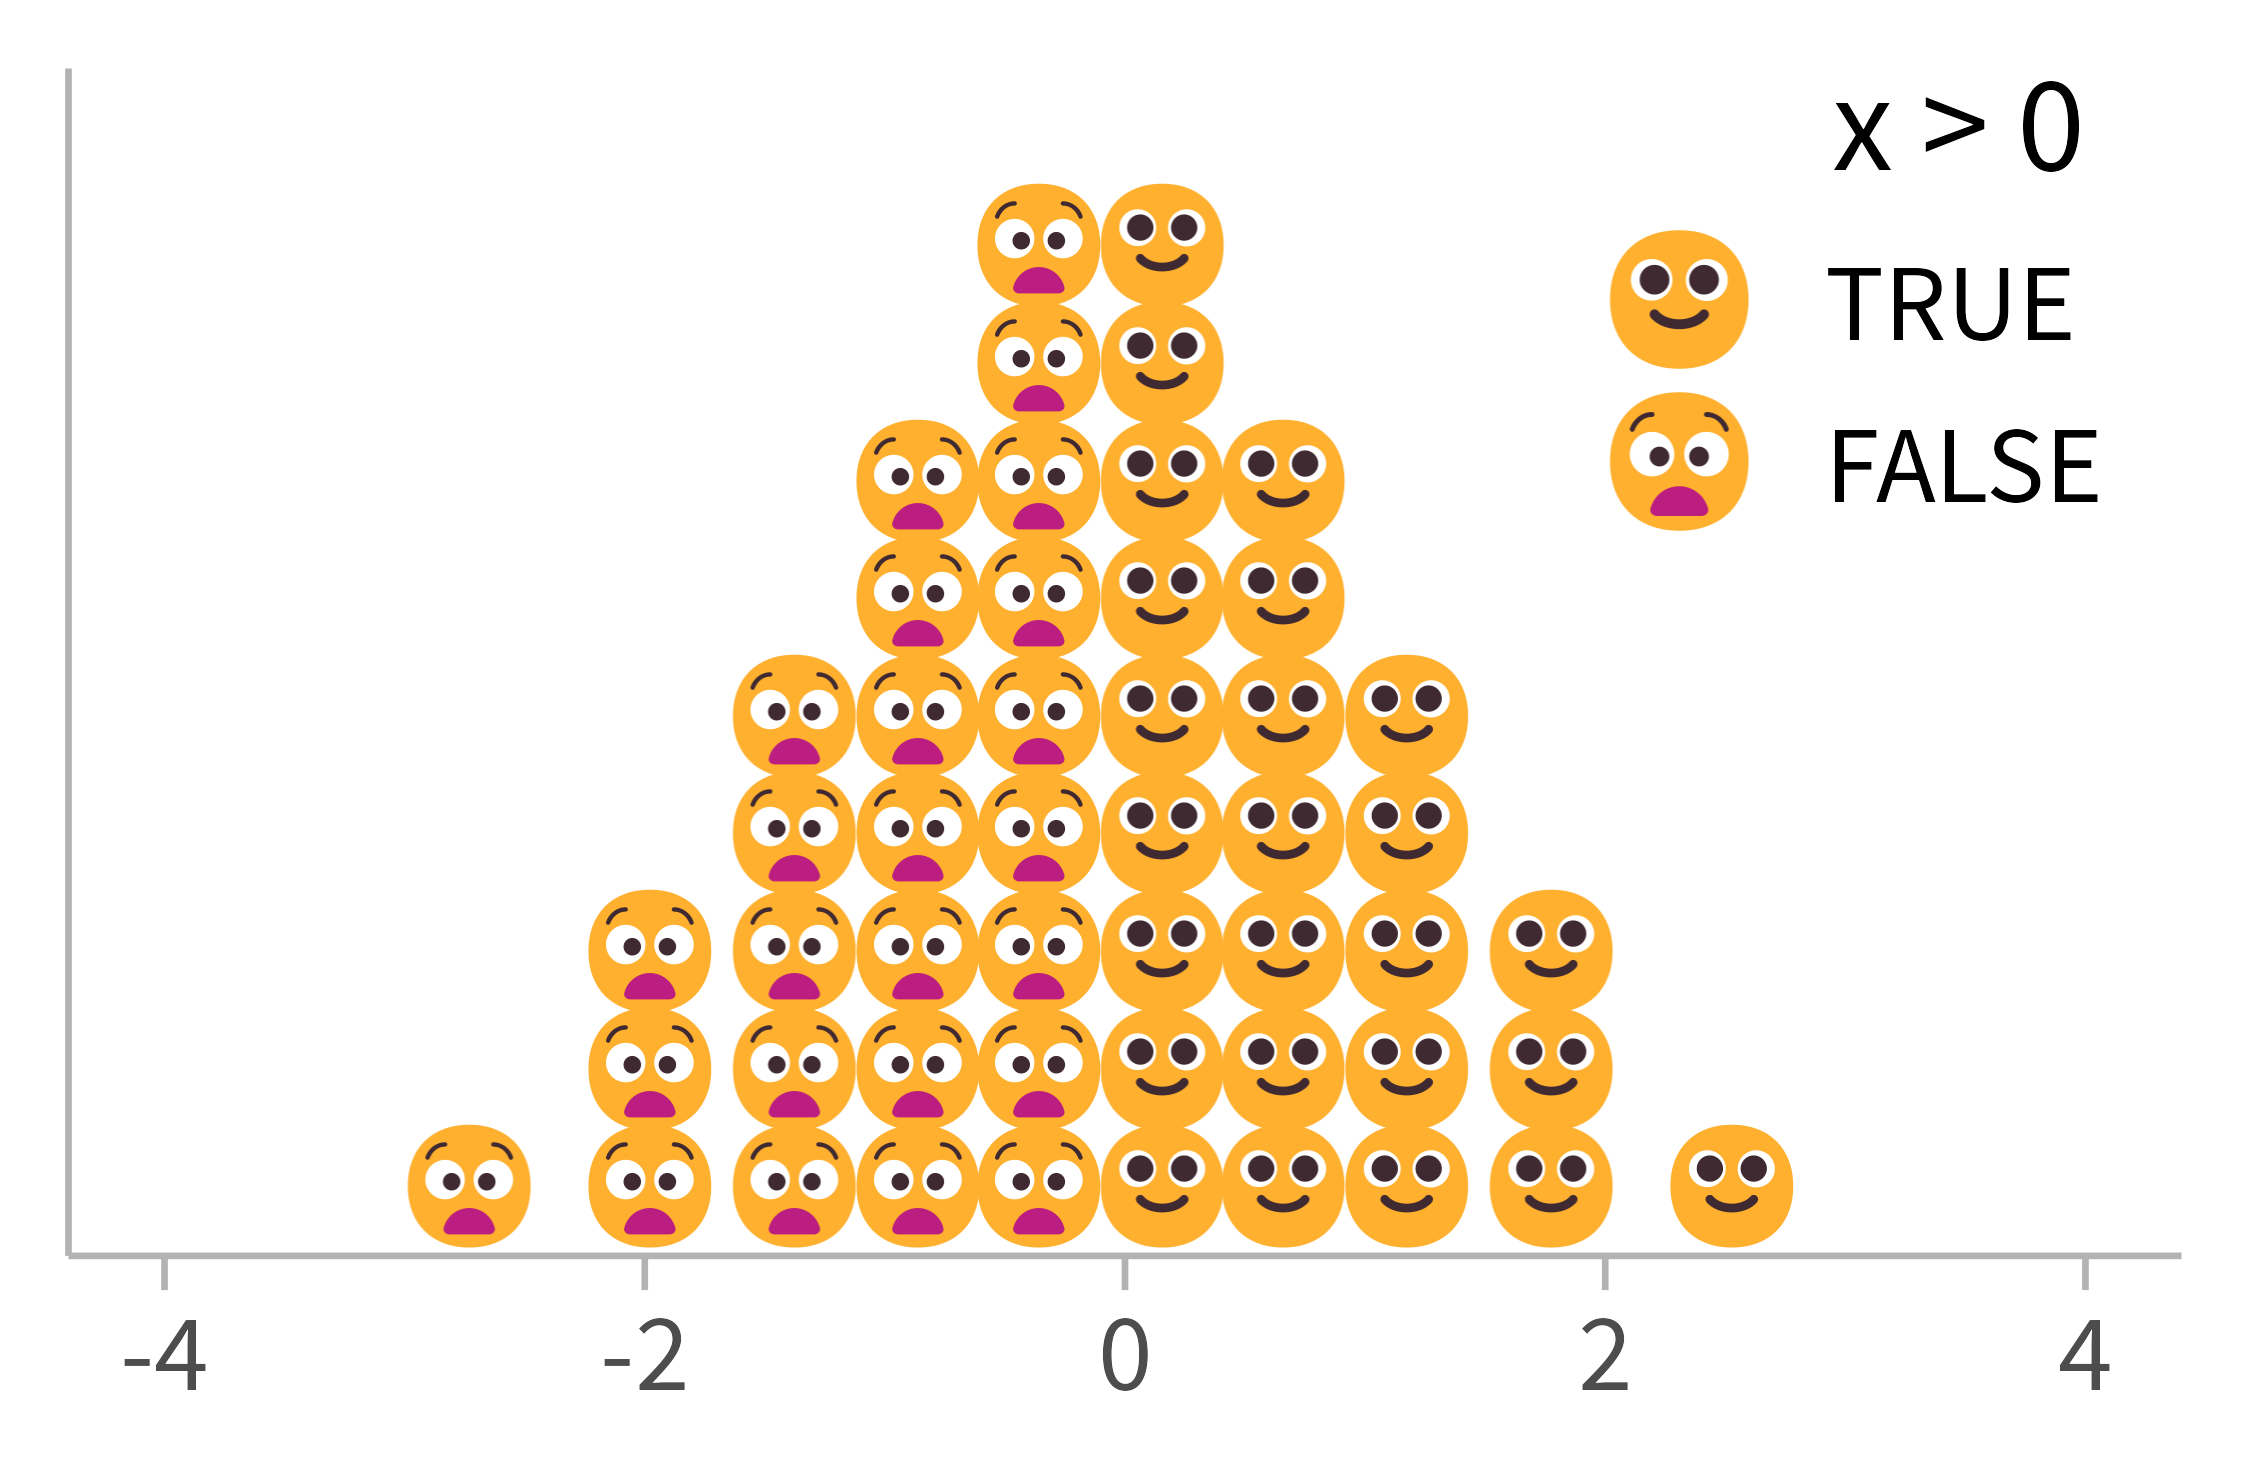
\includegraphics[width=1.2\columnwidth]{figs/3-dots_emoji.png}
  \end{minipage}
\hfill\break

This plot does require specifying what the \textit{shape} scale function is. Abstractly, if we assume each aesthetic mapping \textit{foo} has a scale function $s_\textit{foo}$, we might define the scale function for \textit{shape} as:

\newcommand{\smiley}{\raisebox{-2pt}{
\includegraphics[width=8pt]{emoji-smile.png}}}
\newcommand{\frowny}{\raisebox{-2pt}{
\includegraphics[width=8pt]{emoji-frown.png}}}

\[
s_\textit{shape}(x): x \mapsto \left\{ \begin{array}{ll} \smiley & \textrm{if } x\\ \frowny & \textrm{if }  
 \neg x \end{array} \right.
\]

In \textit{ggplot2} this is:

{
\hfill\break
\small
\centering
\varwidth{\linewidth}
\noindent
\verb|scale_shape_manual(|\\
\verb|  values = c("TRUE" = "|\smiley\verb|", "FALSE" = "|\frowny\verb|")|\\
\verb|)|  
\endvarwidth
\par
\hfill\break
}

This may seem manifestly silly, but there's something to the idea of making discrete outcomes more concrete---or at least more memorable---through graphic depictions, whether it be with emoji or other icons~\cite{haroz2015isotype}. Since arbitrary fonts can be used with \textit{ggplot2} shapes, it is one avenue to creating more expressive dotplots: for example, inspired by \href{https://twitter.com/gdbassett/status/1519067260555513859?s=20}{tweet from Gabe Bassett}, I have used Alberto Cairo's \textit{Wee People} font~\cite{cairo2018weepeople} with \texttt{geom\_dots} to create \href{https://github.com/mjskay/uncertainty-examples/blob/master/weepeople_dotplots.md}{dotplots with anthropomorphic icons} (\cref{fig:teaser}C).

%\subsection{Combinations}

%\textbf{TODO} USGS, Cedric's slab+interval, rainclouds, logit dotplots (plus mention that's in \textit{see}).

\subsection{Further examples}

My hope in the preceding sections was to whet your appetite for the possibilities of an uncertainty visualization grammar grounded in distributions, both of probability and of confidence. I have attempted to give a taste for why ggdist is structured the way it is, its underlying formalism, and how it extends the grammar of graphics in a principled way to support fluid specification of a variety of uncertainty visualizations. What I've shown only scratches the surface of what \textit{ggdist} can do: the interested reader (hopefully you!) can check out the vignettes in the \href{https://mjskay.github.io/ggdist/}{\textit{ggdist} documentation}, which include a slew of examples not covered here. The \href{https://mjskay.github.io/tidybayes/}{\textit{tidybayes} documentation} is also worth checking out, as it includes more examples of the use of \textit{ggdist} with Bayesian models.

\section{Use in the wild}
\label{sec:use-in-the-wild}

%\textbf{TODO} maybe: use in Cedric scherer tutorials, USGS, tidytuesday,   .... ?

I sometimes wonder if the best way to validate visualization ideas is to deploy them into the world and wait to see what happens (as Munzner puts it---to see what users do of their own accord~\cite{munzner2009nested}). Yet, given the vagaries of research project timelines, most systems in \textsc{vis} do not have this luxury---understandably so, lest we wait 10 years to graduate a PhD student. While there are examples of wildly successful systems that came out of visualization research (e.g. \textit{d3}~\cite{bostock2011d3}, \textit{Vega-lite}~\cite{satyanarayan2016vega}), few systems have both the generality and reach of those exemplars. I think \textit{ggdist} falls somewhere in the middle: it has been deployed for several years and enjoys a modest following. This gives me the opportunity to look at some coarse---but naturalistic---data on usage.

\textit{ggdist} currently sees about 14,000 downloads per month from \textsc{cran}~\cite{csardi2019cranlogs} (up from just a few thousand on original launch in 2020, piggy-backing on \textit{tidybayes}' already-established community at the time). Per Google Scholar, it has been cited 46 times (and \textit{tidybayes} 236 times).\footnote{These are all citations of the software itself: neither package has had a paper written about it---yet.} Its Github project has been starred \textasciitilde 620 times, putting it in the company of popular packages like \textit{cowplot} (\textasciitilde 640), \textit{ggalt} (\textasciitilde 630), and \textit{ggtext} (\textasciitilde 600) in the \href{https://exts.ggplot2.tidyverse.org/gallery/}{\textit{ggplot2} extension gallery}. On Github, \textit{ggdist} has 169 issues in its issue tracker, not counting the 305 issues in \textit{tidybayes} (of which many issues prior to \textit{ggdist} splitting from \textit{tidybayes }were \textit{ggdist}-related). Issues especially can be a sign of user engagement, because projects without broader engagement will have issues opened only by the author. To better understand that engagement, I exported all issues from \textit{ggdist} (see \href{https://github.com/mjskay/ggdist/issues}{Github} or the supplement) and read back through them, engaging in a light tagging process based on what I recalled about those issues.

Of the 169 issues on Github, 79 (47\%) were opened by someone other than me; there were 45 unique authors, excluding me. A further 16 issues were opened by me in direct response to some user need, either flowing from a comment on another issue or from a conversation I had with a user on another platform, often Twitter.\footnote{I spend possibly too much time on \texttt{\#rstats} Twitter engaging with data scientists around visualization problems.} Thus, just over half of all issues on \textit{ggdist}'s tracker stem from user engagement with the package---and from a variety of users. I roughly categorized the types of issues (with some overlap) as follows:

\begin{itemize}
    \item 38\%: A request that did (or would) result in a new feature.
    \item 20\%: A user asking for help, usually with a particular plot they are trying to create.
    \item 17\%: A bug.
    \item 16\%: Internal issues, such as code refactoring, cleanup, or \textsc{todo}-tracking.
    \item 9\%: Documentation.
\end{itemize}

Currently, 34 issues (20\%) remain open; only one of these is a bug (recently-reported). 
I have been fortunate to get a wide variety of engagement from users, which has lead to substantive improvement to \textit{ggdist}. It is hard for me to summarize that engagement over all of these issues, but I'll highlight two instances that have had a salient impact on the overall design of \textit{ggdist}, and which also carry some useful lessons for uncertainty visualization in the grammar of graphics.

\textbf{First,} \href{https://github.com/mjskay/ggdist/issues/83}{issue \#83} involves an extensive discussion about how to refactor \textit{ggdist} to merge two classes of \textit{stat}s. Older versions of \textit{ggdist} distinguished between \textit{stat}s designed to summarize distributions represented as vectors of samples (mapped onto \textit{x} or \textit{y}) and those designed to represent distribution objects (mapped onto a now-superceded \textit{dist} aesthetic). My experience answering user issues led me to conclude that this distinction was confusing, so I opened this issue as an attempt to find a better solution. 

Two expert users joined in the discussion, and together we considered a variety of options, including (1) creating a new \textit{distribution} subtype of \textit{x} and \textit{y} scales, similar to the way that continuous values, discrete values, dates, and times are handled by \textit{ggplot2}; or (2) creating new aesthetics, like $x_\textsc{dist}$ and $y_\textsc{dist}$. I prototyped an implementation of the former, realizing some shortcomings: distributions cannot easily be treated as subtypes of positional scales like continuous or discrete variables are, because distributions themselves have subtypes (like being continuous or discrete). In addition, other non-distribution variables must be able to share the same positional scale as the distributional variables: if an \textit{x} scale were given a \textit{continuous distribution} subtype, other merely \textit{continuous} variables (perhaps belonging to other layers in the plot) would no longer work correctly with the scale.

After further discussion, I settled on the $x_\textsc{dist}$ and $y_\textsc{dist}$ design, which makes it easy to intermix distributional objects with non-distributional objects along the same positional scale. This has proven to be a good choice, as I have noticed users struggle less with the new design: previously, the $\textit{dist}$ aesthetic would implicitly be mapped to the relevant positional scale depending on the orientation of the geometry, and this led to confusion when this mapping was not as a user intended. Since the change, I have received feedback from users that the new $x_\textsc{dist}$ and $y_\textsc{dist}$ aesthetics are much easier to use.

\textbf{Second,} \href{https://github.com/mjskay/ggdist/issues/19}{issue \#19}---to automatically detect discrete theoretical distributions and render them correctly as histograms---had been a longstanding wishlist item.\footnote{But who has the time...} About 9 months after I opened it, prompted by a conversation on Twitter, a \textit{ggdist} user posted some examples of plots they might be able to create if the issue were resolved. After a productive brainstorming about the design of discrete distribution displays, I implemented a feature in \textit{ggdist} whereby histograms of discrete theoretical distributions are treated as a type of density plot: a stepped version of their probability mass function is available through the same mappings used for density functions of continuous distributions. This integrates discrete distributions into the same broader framework used to construct other visualization types in \textit{ggdist}, meaning I was able to resolve the issue without creating new special cases for handling discrete distributions from the users' perspective.

Several other issues and features have stemmed from interactions of this kind, including interactions with other R package authors who make use of \textit{ggdist}  (15 other packages, not including \textit{tidybayes}, depend on \textit{ggdist}). Overall, I think \textit{ggdist} has garnered a modest following, and I owe a great debt to community for contributing to its development.

\section{Reflections and lessons learned}

\textit{ggdist} has been under development in some form or another for about six--seven years, and over that time has evolved through user feedback and several waves of refactoring and rewriting. Through all that, I hope I've learned a few things that may be useful for others tackling uncertainty visualization to consider.

\subsection{Distributional notation makes uncertainty visualization much less annoying}

%\textbf{TODO} distributions as core to uncertainty vis, unifying Bayes/freq, power of the syntax itself (making parameters into data, vectorization of arguments to create distributions made the dist+args syntax obsolete, etc)

The core use of distributional visualization to enable a variety of uncertainty visualization types was inspired by our earlier work developing a \textit{Probabilistic Grammar of Graphics} (\textsc{pgog})~\cite{pu2020probabilistic}, which tackled the problem of specifying area and unit visualizations of conditional probability distributions by integrating probability notation into the grammar of graphics. \textsc{pgog} focused mainly on product plots~\cite{wickham2011product}, icon arrays~\cite{ancker2006design}, and dotplots~\cite{wilkinson1999dot}, while \textit{ggdist} expands the expressiveness of a distributional visualization syntax to cover visualization types that are not just functions of density and mass functions, but also functions of \textsc{cdf}s and intervals.\footnote{On the other hand, \textit{ggdist} still does not implement the conditional probability syntax we had in \textsc{pgog}---though the mini-\textsc{dsl} for probability expressions was inspired by it---and it does not support product plots or stacked densities. In a way, \textit{ggdist} has to be more conservative at integrating crazier ideas from research since it has actual users, and also, while the conditional syntax in \textsc{pgog} is elegant for specifying a general class of probabilistic visualizations, its use cases for uncertainty specifically are a little less clear to me. So we'll see.} 

A key insight from working on both \textsc{pgog} and \textit{ggdist} is that bringing notation for probability distributions into the grammar of graphics is a powerful, expressive way to create visualizations of distributions and uncertainty. Iterating on that syntax through user feedback 
(\cref{sec:use-in-the-wild}) has lead to, I think, an approachable but flexible abstraction for uncertainty visualization. A crucial insight---that frequentist uncertainty visualization can be brought into that same framework under the remit of \textit{confidence distributions}~\cite{xie2013confidence}---frees us from multiple tyrannies: (1) endless battles about whether one should be a frequentist or Bayesian when you just want to get on with visualizing your uncertainty; (2) memorizing silly little formulas\footnote{Pedants get one properly typeset ``formul\ae'' per paper. There it was.} for this or that test statistic; (3) implementing different, mutually incompatible, and wholly brittle code paths for visualizing uncertainty under different statistical paradigms. A better world is possible!

\subsection{Balancing abstraction and learnability}

A continual source of tension in the design of \textit{ggdist} has been the balance between abstraction and learnability. At its base, \textit{ggdist} actually only has three geometries, all of which are composite \textit{meta}-geometries: (1) a \textit{slabinterval} geometry, consisting of \textit{slab}, \textit{point}, and \textit{interval} sub-geometries; (2) a \textit{lineribbon} geometry, consisting of \textit{line} and \textit{ribbon} sub-geometries; and (3) a \textit{dotsinterval} geometry, consisting of \textit{dots}, \textit{point}, and \textit{interval} sub-geometries. All other geometries in \textit{ggdist} are \textit{shortcut} geometries, constructed using some combination of default parameters and/or aesthetic mappings applied to one of those three \textit{meta}-geometries.

In principle, \textit{ggdist} could have only those three geometries, but in practice this would not be as usable. First, many specific combinations of options are often used together, so shortcuts for those combinations can save users time. Second, many users will not delve into the depths of \textit{ggdist}'s options to learn how to create each combination they need, and find it easier to remember the name of a shortcut. \textit{ggdist}'s \textit{shortcut} geometries include ones for intervals, eye plots (mirrored slabs with a \textit{pointinterval}), complementary \textsc{cdf} plots, and gradient plots (See \cref{fig:teaser}A). I have found users appreciate these shortcuts, and often ask for more: a raincloud plot shortcut (\cref{fig:teaser}E) is a common request, for example.

In general, I've found users often request shortcuts for creating specific chart types to solve a problem at hand, which is a not unreasonable motivation. However, I have found it productive to hold off on implementing every such request: I usually wait until I can figure out how solving a particular problem (e.g., creating Helske-esque violin-interval plots) can be done within the broader distributional framework in a way that expands the expressiveness of \textit{ggdist} (e.g., allowing interval masses to be mapped onto slab aesthetics). I have also found that extensive documentation and examples can temper the need for quite so many \textit{explicit} shortcuts; an easy-to-adapt example in the documentation acts as a sort of shortcut itself. \textit{ggdist} has extensive long-form \textit{vignettes} that showcase myriad plot types with simple examples. This tension between abstraction and learnability is common to grammar of graphics toolkits: if the ``purest'' form of the grammar of graphics has no chart types at all (per Wilkinson~\cite{wilkinson2012grammar}), but designers often think in terms of chart types~\cite{pu2023inpractice}, how do we best meet them in the middle?

%\textbf{TODO} rainclouds, whwere to draw the line on composite geoms / shortcuts. histograms as slab types or as density estimators. maybe a section on how annoying KDEs are? --- include omething about seeing incorrect vis in the wild, finding good defaults, etc (see also: default points and intervals as median/qi, move to a default KDE that estimates bounds and uses bounded estimator, etc). Maybe something about the various bits of machinery for distributions: discrete/not, determining support, determining bounds when plotting automatically, etc.

%\subsection{faceting versus thickness}

%\textbf{TODO} faceting too awkward, needing thickness for dodging, etc.

\subsection{Uncertainty visualization is tightly coupled with grammar of graphics scales}
\label{sec:jacobians}

As an earlier footnote alluded,\textsuperscript{\ref{foot:jacobians}}   we must be very careful when visualizing density functions. A na\"{i}ve implementation of \texttt{stat\_slab} might simply pass $x$ values through the density function of the distribution mapped to $x_\textsc{dist}$. However, if a non-linear scale transformation is applied, this will result in incorrect densities. This is because, for a random variable $Y = g(X)$, the density function $f_Y$ is:

\[
f_Y(y) = f_X\left(g^{-1}(y)\right) \cdot \left| {g^{-1}}'(y) \right|
\]
In other words, if we have a random variable $X$ that we transform via the function $g$ to get $Y$, we must adjust its density values by the factor $\lvert {g^{-1}}'(y) \rvert$, the absolute value of the derivative of the inverse of $g$. For example if $X$ is drawn from a $\operatorname{log-Normal}(0, 1)$ distribution, we could plot this distribution in base \textit{ggplot2} by using \texttt{ggplot2::stat\_function} combined with R's built-in log-Normal density function, \texttt{dlnorm}:

\noindent
\begin{minipage}{.5\columnwidth}
\small
\begin{verbatim}
ggplot() +
  stat_function(
    fun = \(x) dlnorm(x, 0, 1)
  )
\end{verbatim}
\end{minipage}%
  \begin{minipage}{.4\columnwidth}
    \centering
    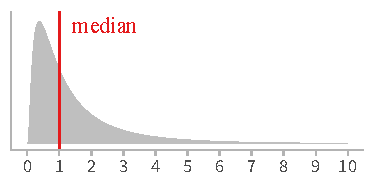
\includegraphics[width=1.2\columnwidth]{figs/3-jacobian-lognorm.pdf}
  \end{minipage}
\hfill\break


If we plot this on a log scale, i.e. plot $Y = \log(X)$, we should hope to see a Gaussian density with a median of $10^0 = 1$ (since medians are preserved under transformation). However, because \textit{ggplot2} has no way to know this function is a density (nor does it necessarily know the derivative of the scale function), the resulting density will be incorrect:

\noindent
\begin{minipage}{.5\columnwidth}
\small
\begin{verbatim}
ggplot() +
  stat_function(
    fun = \(x) dlnorm(x, 0, 1)
  ) +
  scale_x_log10()
\end{verbatim}
\end{minipage}%
  \begin{minipage}{.4\columnwidth}
    \centering
    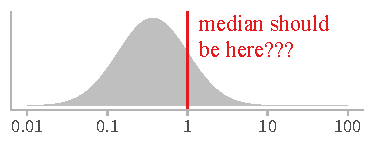
\includegraphics[width=1.2\columnwidth]{figs/3-jacobian-incorrect.pdf}
  \end{minipage}
\hfill\break

The line at 1 does not divide the area into two regions with equal mass, as it would if it were the median. I have no doubt this has led to errors amongst \textit{ggplot2} users.\footnote{For example, \textit{ggplot2} \href{https://github.com/tidyverse/ggplot2/issues/4783}{issue \#4783} is written by a user asking why a theoretical density and samples from a distribution do not line up under transformation---a less attentive user may never have noticed.} Fortunately, \textit{ggdist} does know how to correctly transform densities. It uses a combination of symbolic and (as a fallback) numeric methods to calculate derivatives of \textit{ggplot2} scale transformations to adjust densities.\footnote{Specifically, \textit{ggdist} applies R's built-in \texttt{D} function to get the symbolic derivative of the expression defining the scale function and, if that fails, uses \texttt{numDeriv::jacobian}~\cite{gilbert2016numderiv}. In the future, if my \href{https://github.com/r-lib/scales/pull/341}{pull request \#341} to the \textit{scales} package is accepted, derivatives of scale functions will be offloaded into the guts of \textit{ggplot2} and simultaneously made more reliable.} As a result, we can visualize a log-transformed log-Normal density and get the correct result:

\noindent
\begin{minipage}{.5\columnwidth}
\small
\begin{verbatim}
ggplot() +
  aes(xdist = dist_lognormal(0,1)) +
  stat_slab() +
  scale_x_log10()
\end{verbatim}
\end{minipage}%
  \begin{minipage}{.4\columnwidth}
    \centering
    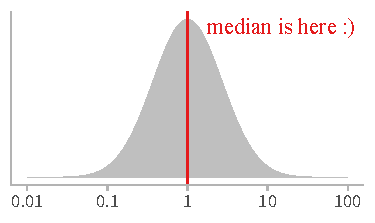
\includegraphics[width=1.2\columnwidth]{figs/3-jacobian-correct.pdf}
  \end{minipage}
\hfill\break

This emphasizes the need for uncertainty visualization systems to be \textit{scale-aware}: it is not possible to comprehensively implement uncertainty visualization purely as a data pre-processing step.\footnote{It also suggests that grammar of graphics systems should implement derivatives as part of their scale transformation functions.} This is one example of what Xiaoying Pu and I\footnote{Let's be honest, Xiaoying did all the hard work.} termed a \textit{tight coupling} of data transformation and visualization specification in a study of expert \textit{ggplot2} users~\cite{pu2023inpractice}: the data processing (calculating the density) is tightly coupled with the visualization spec (the scale transformation), and these must be kept in sync. Moving the specification of densities into the visualization spec itself is one way to ensure this, eliminating a whole class of errors. 


\subsection{Where to go from here}

I would hardly deign to pretend \textit{ggdist} has solved all of uncertainty visualization. In truth, it's stuck to a well-defined corner of it: largely univariate uncertainty visualization; although \textit{lineribbon} supports some multivariate stuff: besides being able to visualize many conditional distributions at once as ribbons, it can visualize joint uncertainty bands in the style of functional boxplots~\cite{sun2011functional,mirzargar2014curve,juul2021fixed} by using the \texttt{curve\_interval} function.\footnote{See examples at \href{https://mjskay.github.io/ggdist/articles/lineribbon.html\#curve-boxplots-aka-lineribbons-with-joint-intervals-or-curvewise-intervals}{the end of the lineribbon vignette}.} Obvious extensions include two-dimensional densities, for which support exists in \textit{ggplot2} but which is not built around the same framework of distributional functions and objects \textit{ggdist} is. Thus, ripe for integration and extension.

Thinking further afield, there are other types of uncertainty visualizations not well-supported in \textit{ggdist}, or which \textit{ggdist}'s abstractions are not relevant to. One obvious example is spaghetti plots~\cite{cox2013visualizing,liu2018visualizing}---though, if you already have a joint sample from a distribution of paths in a long-format data frame, \textit{ggplot2} makes it trivial to visualize this. Similarly, animated hypothetical outcome plots (\textsc{hop}s)~\cite{hullman2015hypothetical,kale2018hypothetical} are straightforward to construct using \textit{ggplot2} with the \textit{gganimate} package. A more interesting question might be: if one designed a new uncertainty visualization grammar from the ground up to support all of the  visualizations in \textit{ggdist} and \textsc{pgog}, plus static sample-based visualizations like spaghetti plots and animated sample-based \textsc{hop}s, what would it look like? Can a coherent framework bring all of these ideas together, and suggest new ideas too? I am hopeful it can.

\section{Conclusion}

\textit{ggdist} has been a six-year journey in implementing a distributional, petty-statistics-camp-agnostic approach to uncertainty visualization in the grammar of graphics. While there remain many interesting future challenges to integrating further classes of uncertainty visualizations under one umbrella, the flexibility and expressiveness of \textit{ggdist} thus far demonstrates the power of its underlying abstractions. Taking a step back, it also shows the value of continuing to push more aspects of visualization specification into the formal description of the visualization itself, both by enabling a wider range of visualization types to be easily created and by reducing the potential for certain classes of errors.\footnote{Potential we also saw in reducing errors with incorrect normalization of conditional probability distributions in \textsc{pgog}~\cite{pu2020probabilistic} or in keeping data transformation and visualization specification code in sync more generally in \textit{ggplot2}~\cite{pu2023inpractice}.} 

\section*{Supplemental Materials}
\label{sec:supplemental_materials}

Supplemental materials, released under a CC-BY 4.0 license, are available on GitHub (\href{https://github.com/mjskay/ggdist-paper}{github.com/mjskay/ggdist-paper}) and archived on Zenodo (\href{https://doi.org/10.5281/zenodo.7770984}{doi:10.5281/zenodo.7770984}).
Materials include: (1) an RMarkdown file that generates the figures in the paper; (2) generated figure images; (3) a tagged archive of \textit{ggdist} Github issues; (4) an RMarkdown file calculating some descriptive statistics of \textit{ggdist} Github isses; and (5) the full source of this paper.

The full source of \textit{ggdist}, released under a GPL 3.0 license, is available on GitHub (\href{https://github.com/mjskay/ggdist}{github.com/mjskay/ggdist}) and archived on Zenodo (\href{https://doi.org/10.5281/zenodo.3879620}{doi:10.5281/zenodo.3879620}). \textit{ggdist} may also be installed from \textsc{cran} via the R command \texttt{install.packages("ggdist")}.

\section*{Figure Credits}
\label{sec:figure_credits}

All figures were created by Matthew Kay and are released under a CC-BY 4.0 license.

%% if specified like this the section will be ommitted in review mode
\acknowledgments{%
I would like to thank various folks who have used, given feedback on, or contributed to \textit{ggdist} over the years (this list is neither exhaustive nor in any particular order): Xiaoying Pu, Alex Kale, Abhraneel Sarma, Fumeng Yang, Matti Vuorre, Dominique Makowski, TJ Mahr, Tim Mastny, Aki Vehtari, Brenton M. Wiernik, Arthur Albuquerque, A. Solomon Kurz, Gabe Bassett, Mitchell O'Hara-Wild, Steve Haroz, Jarrett Byrnes, Dylan H. Morris, Dmytro Perepolkin, C\'edric Scherer,  Isabella Ghement, Teun van den Brand, and Jonas Kristoffer Lindeløv. This work was supported in part by NSF award IIS-1910431.%
}


\bibliographystyle{abbrv-doi}
%\bibliographystyle{abbrv-doi-hyperref-narrow}
%\bibliographystyle{abbrv-doi}
%\bibliographystyle{abbrv-doi-narrow}

\bibliography{template}


%% ^^^^^   FOR IEEE VIS, EVERYTHING HERE MAY BE INCLUDED IN THE    ^^^^^ %%
%% 2-PAGE ALLOTMENT FOR REFERENCES, FIGURE CREDITS, AND ACKNOWLEDGEMENTS %%

\appendix % You can use the `hideappendix` class option to skip everything after \appendix


\end{document}

